\documentclass{beamer}

% Theme choice
\usetheme{Madrid}

% Packages
\usepackage{amsmath, amssymb, graphicx, listings}

% Title Page
\title{Bilinear Transformation}
\author{Nithin.K}
\date{\today}

\begin{document}

\begin{frame}
	\titlepage
\end{frame}

\begin{frame}{Problem Statement}
	\textbf{Given Differential Equation:}
	\begin{align}
		\frac{d^2y}{dx^2} + 1 &= 0
	\end{align}
	\textbf{Initial Conditions:}
	\begin{align}
		y(0) &= 0, \quad y'(0) = 0
	\end{align}
\end{frame}

\begin{frame}{Laplace Transform Method}
	\textbf{Laplace Transform:}
	\begin{align}
		\mathcal{L}\{f(t)\} &= \int_{0}^{\infty} e^{-st} f(t) \, dt
	\end{align}
	\textbf{Properties:}
	\begin{align}
		\mathcal{L}\{y''\} &= s^2 \mathcal{L}\{y\} - s y(0) - y'(0) \\
	\end{align}
	\begin{align}
		\mathcal{L}\{1\} &= \frac{1}{s}
	\end{align}
	\begin{align}
		\mathcal{L}^{-1}\left(\frac{2}{s^3}\right) &= x^2 u(x)
	\end{align}
	\textbf{Substituting the initial conditions gives}
	\begin{align}
		y'' + 1 = 0
	\end{align}
	\begin{align}
		\mathcal{L}\{y''\} + \mathcal{L}\{1\} = 0
	\end{align}
\end{frame}

\begin{frame}{Inverse Laplace Transform}
        \begin{align}
	        s^2 \mathcal{L}\{y\} - sy\left(0\right) - y'\left(0\right) + \frac{1}{s} = 0
	\end{align}
	\begin{align}
	        \mathcal{L}\{y\} = \frac{-1}{s^3}
	\end{align}
	\begin{align}
	         y = \frac{-x^2}{2}u\left(x\right)
	\end{align}
\end{frame}

\begin{frame}{Bilinear Transform}
	\textbf{Mapping to z-domain:}
	\begin{align}
		s = \frac{2}{h} \left(\frac{1 - z^{-1}}{1 + z^{-1}} \right)
	\end{align}
	\textbf{Substituting:}
	\begin{align}
		Y(z) &= -\left(\frac{h}{2}\right)^3 \left(\frac{1 + 3z^{-1} + 3z^{-2} + z^{-3}}{1 - 3z^{-1} + 3z^{-2} - z^{-3}} \right)
	\end{align}
	Multiply the above equation by $z^3$ and taking the inverse z-transform yields the difference equation: \\
	ROC: $z \neq 0$ \\
	\textbf{Difference Equation:}
	\begin{align}
		y(n+3) &= -3y(n+1) + y(n) + 3y(n+2) + h^2\delta(n) - \left(\frac{h}{2}\right)^3\delta(n)
	\end{align}
\end{frame}

\begin{frame}{Finite Difference Approximation}
	\textbf{Second Derivative Approximation:}
	\begin{align}
		\frac{d^2y}{dx^2} &\approx \frac{y_{n+1} - 2y_n + y_{n-1}}{h^2}
	\end{align}
	\textbf{Substituting:}
	\begin{align}
		y_{n+1} &= 2y_n - y_{n-1} - h^2
	\end{align}
	\textbf{Initial Conditions:}
	\begin{align}
		y_0 &= 0, \quad y_1 = 0
	\end{align}
\end{frame}

\begin{frame}{Plot of the Solution}
	\centering
	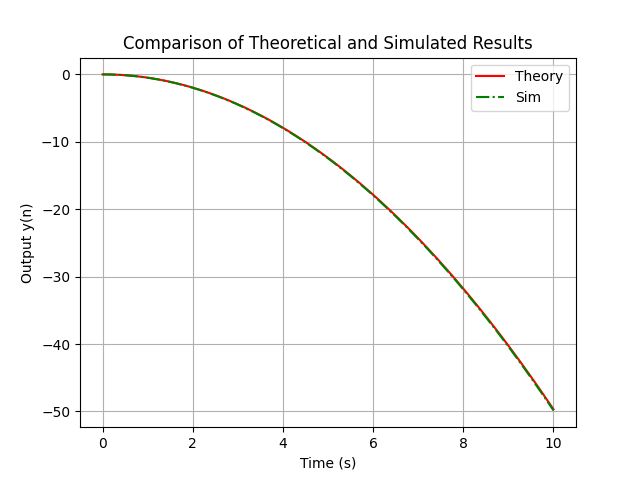
\includegraphics[width=0.8\textwidth]{figs/fig.png}
\end{frame}

\begin{frame}{Conclusion}
	\begin{itemize}
		\item Laplace Transform provides an analytical solution.
		\item Bilinear Transform maps it to the z-domain for digital processing.
		\item Finite Difference Method allows computational approximation.
		\item \footnotesize Reference : https://github.com/nithin769/EE1030/sciprogramming/question-9.3.11.3/codes
	\end{itemize}
\end{frame}

\end{document}

